
\documentclass[12pt,a4paper]{report}

% Pachete de bază
\usepackage{iftex}
\ifPDFTeX
  \usepackage[utf8]{inputenc}
  \usepackage[T1]{fontenc}
  \usepackage{lmodern}
\else
  \usepackage{fontspec}
  \setmainfont{lmroman10-regular.otf}[
    BoldFont = lmroman10-bold.otf,
    ItalicFont = lmroman10-italic.otf,
    BoldItalicFont = lmroman10-bolditalic.otf
  ]
  \setsansfont{lmsans10-regular.otf}[
    BoldFont = lmsans10-bold.otf,
    ItalicFont = lmsans10-oblique.otf
  ]
  \setmonofont{lmmono10-regular.otf}
\fi
\usepackage[romanian]{babel}
\usepackage{microtype}
\usepackage[left=3cm,textwidth=15cm,top=3cm,textheight=22cm]{geometry}

% Matematică, imagini și diagrame
\usepackage{amsmath}
\usepackage{graphicx}
\usepackage{float}

% Link-uri
\usepackage[hidelinks]{hyperref}

% Denumiri în română
\addto\captionsromanian{%
  \renewcommand{\contentsname}{Cuprins}%
  \renewcommand{\listfigurename}{Lista figurilor}%
  \renewcommand{\listtablename}{Lista tabelelor}%
  \renewcommand{\figurename}{Figura}%
  \renewcommand{\tablename}{Tabelul}%
  \renewcommand{\partname}{Partea}%
  \renewcommand{\chaptername}{Capitolul}%
  \renewcommand{\bibname}{Bibliografie}%
  \renewcommand{\appendixname}{Anexa}%
}

% Include imaginea dacă există; altfel lasă spațiu gol și nu oprește compilarea.
\newcommand{\safeincludegraphics}[2][]{%
  \IfFileExists{#2}{\includegraphics[#1]{#2}}{%
    \vspace{100pt}%
  }%
}

\newcommand{\diagramplaceholder}[1]{%
  \fbox{%
    \parbox[c][5cm][c]{0.82\textwidth}{%
      \centering #1%
    }%
  }%
}

\begin{document}
\selectlanguage{romanian}
\sloppy

\thispagestyle{empty}

\begin{center}

	\begin{figure}[h!]\vspace{-20pt}
		\begin{center}
			\safeincludegraphics[width=100pt]{FI.png}
		\end{center}

	\end{figure}


	{\large{\bf UNIVERSITATEA DE VEST DIN TIMIȘOARA

		FACULTATEA DE INFORMATICĂ

		PROGRAMUL DE STUDII DE LICENȚĂ: Informatică }}

	\vspace{120pt}{\huge {\bf LUCRARE DE LICENȚĂ }}

	\vspace{150pt}
\end{center}


{\large\noindent{\bf COORDONATOR:\hfill ABSOLVENT:}

\noindent Lector Dr. Popovici Adriana \hfill Preda Slavoliub-Denis}


\vfill

\begin{center}
	{\bf TIMIȘOARA

		2026}
\end{center}

\newpage
\thispagestyle{empty}

\begin{center}
	{\large{\bf UNIVERSITATEA DE VEST DIN TIMIȘOARA

			FACULTATEA DE INFORMATICĂ

			PROGRAMUL DE STUDII DE LICENȚĂ: Informatică }}

	\vspace{120pt}{\huge {\bf Dezvoltarea unei platforme web de management al proiectelor cu funcționalități asistate de inteligența artificială}}

	\vspace{150pt}
\end{center}


{\large\noindent{\bf COORDONATOR:\hfill ABSOLVENT:}

\noindent Lector Dr. Popovici Adriana \hfill Preda Slavoliub-Denis}


\vfill

\begin{center}
	{\bf TIMIȘOARA

		2026}
\end{center}

\newpage\normalsize{}

\clearpage
\thispagestyle{plain}


\cleardoublepage


\cleardoublepage\chapter*{Abstract}
\thispagestyle{plain}

This thesis presents the design and implementation of \textit{SDLC Hub}, a web platform for software project management. The application addresses a practical problem encountered in software teams: the need to work with different methodologies, preserve decision traceability, and connect development activity from GitHub with planning and project monitoring.

SDLC Hub supports Scrum, Kanban, and Scrumban. The selected methodology is not treated as a simple label: depending on the project mode, the interface, permissions, backlog, sprints, estimation fields, and reports are adapted dynamically. The application includes authentication, projects, roles, permissions, tasks, subtasks, comments, board, backlog, sprints, calendar, notifications, internal documentation, reporting, GitHub integration, real-time collaboration, and global administration.

An important contribution is the integration of AI-assisted features into concrete workflows: methodology recommendation, requirements refinement, story point estimation, risk analysis, workload balancing, and release notes generation. The thesis presents the motivation behind the application, related project management tools, the main requirements, the graphical interface, the architecture, the data model, the implementation details, and the validation of the implemented features.

\cleardoublepage\setcounter{tocdepth}{2}\setcounter{secnumdepth}{3}
\tableofcontents
\cleardoublepage
\listoffigures

\cleardoublepage


\chapter{Introducere}
\label{chap:introducere}

\section{Studiu contextual}
Managementul proiectelor software reprezintă o componentă importantă a ciclului de viață al dezvoltării software. O echipă care construiește un produs informatic trebuie să poată transforma cerințele în activități concrete, să urmărească progresul, să colaboreze, să controleze schimbările și să păstreze o evidență a deciziilor luate. În acest context, instrumentul de management folosit de echipă nu este doar o listă de task-uri, ci un spațiu în care planificarea, execuția, comunicarea și raportarea se întâlnesc.

În practică, echipele software nu lucrează toate după aceeași metodologie. Scrum organizează munca în sprinturi, roluri, evenimente și artefacte, punând accent pe planificare iterativă și inspecție regulată \cite{scrumguide2020}. Kanban pune accent pe vizualizarea fluxului de lucru, limitarea lucrului în desfășurare și îmbunătățirea continuă a procesului \cite{kanbanguide2020}. Între aceste două direcții apare Scrumban, o abordare hibridă care permite folosirea unor elemente de planificare din Scrum împreună cu o execuție mai flexibilă, apropiată de Kanban.

Pe lângă metodologia aleasă, echipele au nevoie de trasabilitate. Un task poate fi creat dintr-o cerință, poate fi discutat în comentarii, poate fi estimat, mutat pe board, implementat într-un branch GitHub și finalizat printr-un pull request. Dacă aceste informații se află în instrumente separate, contextul se pierde ușor. De aceea, o platformă modernă trebuie să lege activitatea de management de activitatea tehnică și să permită urmărirea întregului traseu al muncii.

În ultimii ani, inteligența artificială a început să fie folosită tot mai des în activități de dezvoltare software, inclusiv pentru analiză, sumarizare, rafinare de cerințe și estimări \cite{mahboob2024future}. Totuși, aceste funcții sunt utile doar dacă sunt integrate într-un flux real. O sugestie AI izolată, plasată într-o pagină separată, nu ajută suficient echipa. În schimb, dacă AI-ul apare în momentul în care utilizatorul creează un proiect, rafinează o cerință, estimează un task sau analizează un risc, valoarea lui devine practică.

\section{Motivație}
Motivația acestei lucrări pornește de la observația că multe aplicații de management al proiectelor sunt fie foarte complexe, fie prea simple pentru un flux software complet. O aplicație complexă poate oferi multe opțiuni, dar configurarea ei poate fi dificilă pentru o echipă mică sau pentru un proiect universitar. O aplicație simplă este ușor de folosit, dar nu oferă întotdeauna roluri, permisiuni, audit, rapoarte, documentație internă sau integrare cu activitatea din cod.

O altă motivație este flexibilitatea metodologică. Într-un proiect real, echipa poate începe cu Scrum, poate observa că are nevoie de un flux continuu și poate trece spre Kanban sau Scrumban. Dacă aplicația tratează metodologia doar ca etichetă, schimbarea nu are efect real. Dacă metodologia controlează paginile, câmpurile, regulile și rapoartele, instrumentul devine mai apropiat de modul real de lucru al echipei.

Lucrarea urmărește realizarea unei platforme web care să combine managementul proiectelor software, adaptarea la metodologii agile și funcționalități asistate de inteligența artificială. Scopul nu este reproducerea completă a unui produs enterprise matur, ci construirea unei aplicații coerente, demonstrabile, în care principalele fluxuri de lucru pot fi parcurse de la început până la final.

\section{Descriere}
Soluția propusă este \textit{SDLC Hub}, o platformă web pentru managementul proiectelor software. Utilizatorul poate crea cont, se poate autentifica, poate crea un proiect sau poate intra într-un proiect existent. La crearea proiectului, aplicația oferă un wizard care ajută la definirea identității proiectului, alegerea metodologiei, configurarea rolurilor și pregătirea integrării DevOps.

Aplicația suportă Scrum, Kanban și Scrumban. Metodologia selectată influențează interfața și regulile sistemului. Pentru Scrum și Scrumban sunt disponibile backlog-ul și sprinturile, iar pentru Kanban accentul cade pe board și pe flux continuu. Schimbarea metodologiei este controlată prin preview, blocaje, avertismente și audit log.

SDLC Hub include module pentru task-uri, subtasks, comentarii, board, backlog, sprinturi, roluri, permisiuni, audit, calendar, notificări, documentație internă, rapoarte, workload, integrare GitHub, suport, administrare globală și funcționalități AI. Backend-ul este construit cu FastAPI, SQLAlchemy, Alembic și PostgreSQL, iar frontend-ul folosește Next.js, React, TypeScript și Tailwind CSS. Comunicarea dintre frontend și backend se face prin API REST, iar actualizările live sunt realizate prin WebSocket.


\chapter{Aplicații similare}
\label{chap:problematica}

\section{Jira Software}
Jira Software este una dintre cele mai cunoscute aplicații pentru managementul proiectelor și este dezvoltată de Atlassian. Pagina oficială de funcționalități prezintă Jira ca instrument pentru planificare, urmărirea progresului, colaborare, automatizare de workflow și raportare \cite{atlassianjira}. Jira oferă mai multe tipuri de vizualizări, precum board, listă, calendar și timeline, iar pentru echipele software include funcții utile pentru sprinturi, rapoarte, dependențe, câmpuri configurabile și integrări.

\begin{figure}[H]
\centering
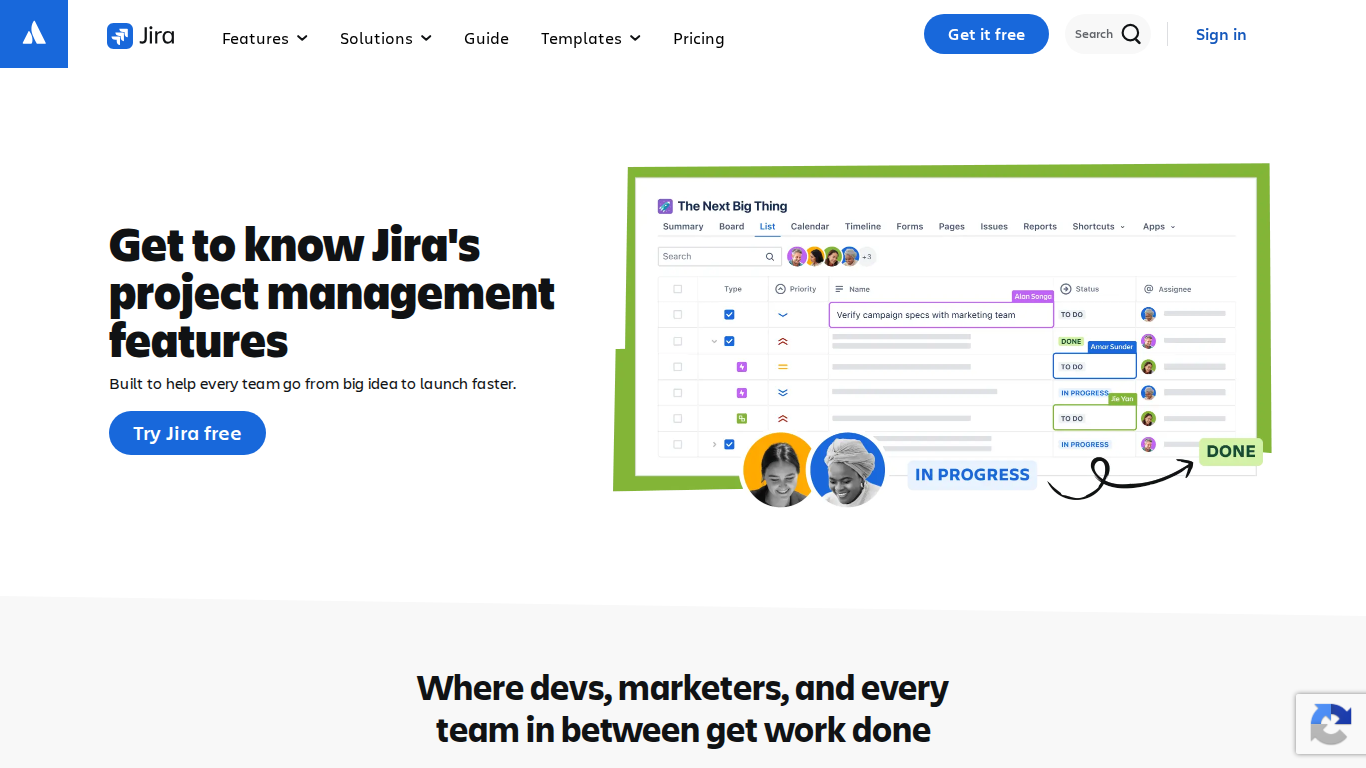
\includegraphics[width=0.9\textwidth]{figures/related-jira.png}
\caption{Interfață Jira Software, conform paginii oficiale Atlassian \cite{atlassianjira}}
\label{fig:jira-ui}
\end{figure}

\textbf{Avantaje.} Principalul avantaj al Jira este nivelul ridicat de configurare. Platforma permite definirea de workflow-uri, câmpuri, permisiuni, rapoarte și integrări, fiind potrivită pentru organizații care au procese complexe. Jira este puternică și prin ecosistemul Atlassian, deoarece se poate conecta cu alte instrumente precum Confluence, Bitbucket sau aplicații din Atlassian Marketplace.

\textbf{Dezavantaje.} Complexitatea poate deveni o problemă pentru echipe mici sau pentru proiecte care au nevoie de configurare rapidă. Multe funcții sunt utile, dar pot încărca experiența utilizatorului. Din perspectiva SDLC Hub, Jira este un reper important pentru board, sprint management și raportare, însă aplicația propusă urmărește o experiență mai directă, cu tranziție explicită între Scrum, Kanban și Scrumban.

\section{Trello}
Trello este o aplicație orientată spre organizare vizuală prin board-uri, liste și carduri. Ghidul oficial Trello descrie procesul de început ca fiind simplu: utilizatorul se înregistrează, creează un board și poate începe să organizeze munca echipei \cite{trello}. Trello include funcții precum template-uri, automatizări, Power-Ups, integrări, planificare și mai multe moduri de folosire pentru echipe diferite.

\begin{figure}[H]
\centering
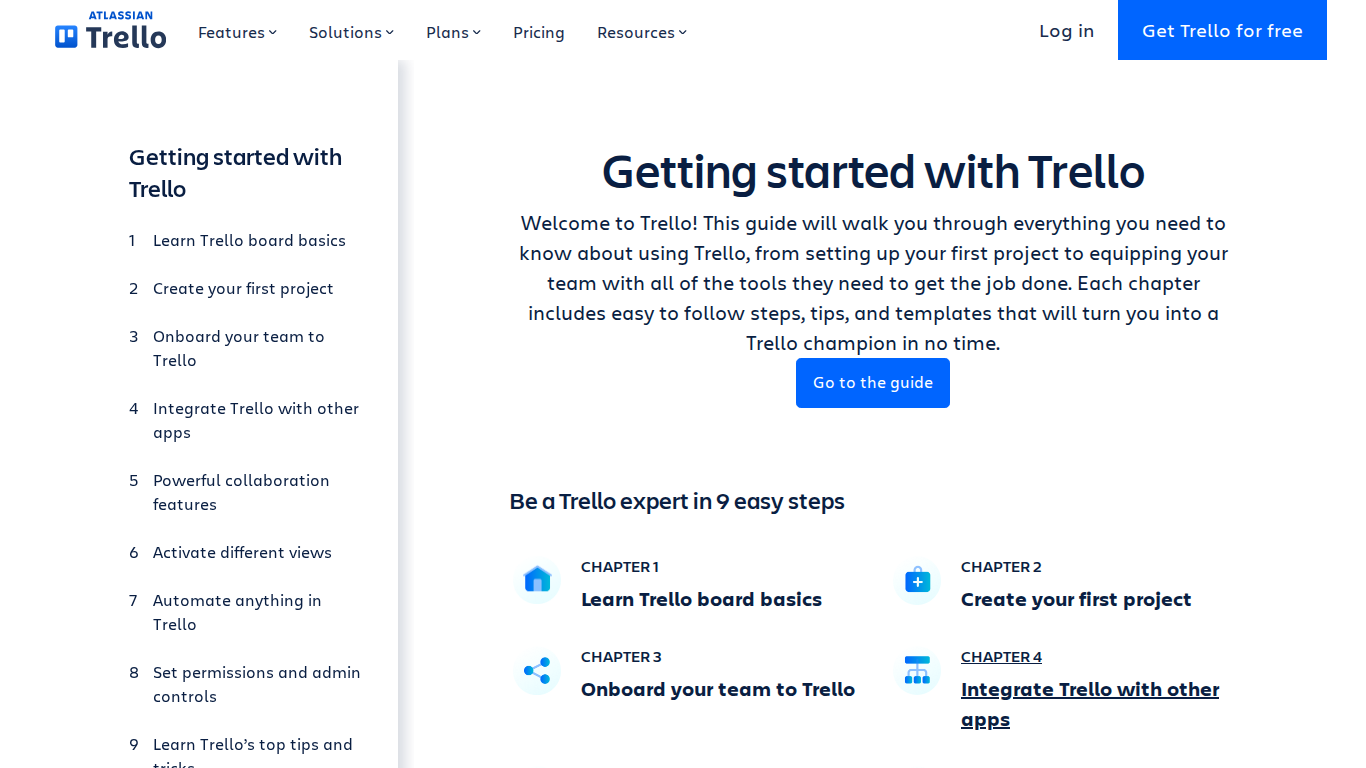
\includegraphics[width=0.9\textwidth]{figures/related-trello.png}
\caption{Pagina oficială Trello Guide \cite{trello}}
\label{fig:trello-ui}
\end{figure}

\textbf{Avantaje.} Trello este ușor de înțeles și de folosit. Metafora cardurilor mutate între liste este naturală pentru utilizatori și se potrivește foarte bine cu un flux Kanban simplu. Platforma este potrivită pentru echipe mici, proiecte personale și activități unde vizibilitatea rapidă este mai importantă decât configurarea avansată.

\textbf{Dezavantaje.} Trello nu este construit special pentru toate nevoile unui proces software complet. Auditul detaliat, permisiunile granulare, sprint management-ul, rapoartele agile și integrarea profundă cu task-uri tehnice necesită extensii sau soluții suplimentare. SDLC Hub păstrează claritatea vizuală a unui board, dar adaugă roluri, metodologii, audit, rapoarte, documentație și integrare DevOps.

\section{GitHub Projects}
GitHub Projects este integrat în ecosistemul GitHub și permite planificarea muncii direct lângă issues și pull request-uri. Documentația oficială descrie Projects ca un instrument flexibil pentru planificare și urmărirea muncii, bazat pe tabele, board-uri și roadmap-uri \cite{githubprojects}. Proiectele pot avea vizualizări personalizate, filtre, câmpuri custom, grafice, template-uri și automatizări.

\begin{figure}[H]
\centering
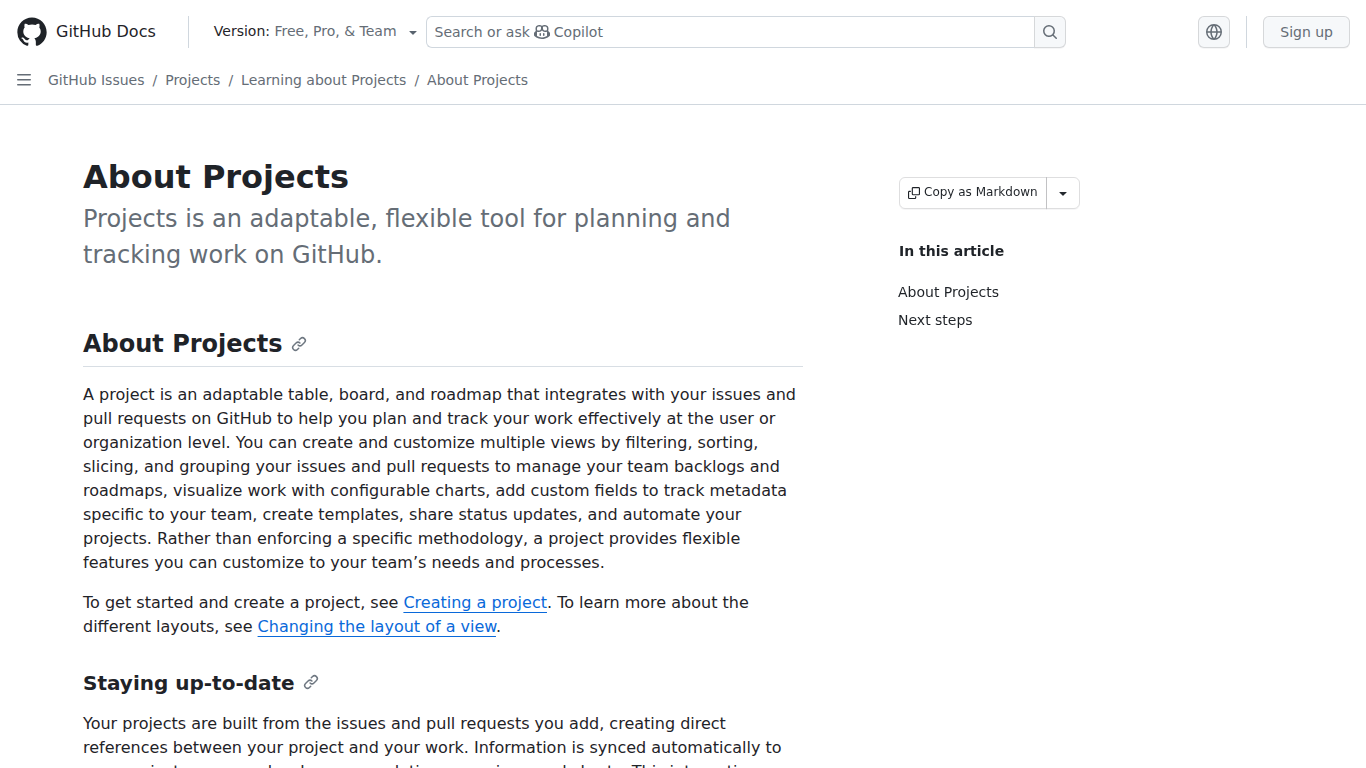
\includegraphics[width=0.9\textwidth]{figures/related-github-projects.png}
\caption{Documentația oficială GitHub Projects \cite{githubprojects}}
\label{fig:github-projects-ui}
\end{figure}

\textbf{Avantaje.} Cel mai mare avantaj este apropierea de cod. Issues, pull request-urile și proiectele sunt conectate, iar actualizările pot fi sincronizate între ele. Pentru echipe tehnice, această apropiere reduce distanța dintre planificare și implementare. GitHub Projects este util și prin flexibilitatea vizualizărilor: tabel, board și roadmap.

\textbf{Dezavantaje.} GitHub Projects este mai puțin accesibil pentru utilizatori non-tehnici și nu tratează managementul proiectului ca spațiu separat de repository. Rapoartele, rolurile de proiect, tranzițiile metodologice și funcțiile AI nu sunt elemente centrale ale aplicației. SDLC Hub preia ideea de trasabilitate între task și cod prin webhook-uri GitHub, dar păstrează managementul proiectului într-o platformă dedicată.

\section{Analiză critică}
Jira, Trello și GitHub Projects acoperă direcții importante. Jira este foarte configurabilă, Trello este simplă și vizuală, iar GitHub Projects este aproape de cod. Totuși, fiecare aplicație are și limite. Jira poate deveni dificilă pentru echipe mici, Trello nu acoperă suficient un proces software complet, iar GitHub Projects este strâns legat de repository și de utilizatori tehnici.

SDLC Hub este construit pornind de la aceste observații. Aplicația propusă preia ideea de board vizual, dar o leagă de task-uri, sprinturi, roluri, permisiuni și audit. Preia ideea de apropiere de cod, dar prin webhooks și evenimente GitHub, nu prin mutarea întregului management în repository. Preia ideea de raportare, dar o adaptează metodologiei active. În plus, metodologia nu este doar un câmp informativ, ci influențează paginile și regulile aplicației. Studiile comparative asupra Scrum și Kanban arată că modul de lucru poate influența performanța proiectelor software \cite{lei2017statistical}, motiv pentru care metodologia trebuie tratată ca parte activă a sistemului.


\chapter{Descrierea aplicației SDLC Hub}
\label{chap:descriere-aplicatie}

\section{Cerințele aplicației}
Principalele cerințe ale aplicației sunt ca un utilizator să poată crea un cont, să se autentifice, să creeze un proiect, să aleagă o metodologie, să invite membri, să gestioneze task-uri și să urmărească progresul proiectului. Aplicația trebuie să ofere un flux complet pentru echipe software, nu doar o pagină de board. Din acest motiv, SDLC Hub include și roluri, permisiuni, sprinturi, calendar, documentație, notificări, rapoarte, workload, integrare GitHub și funcții AI.

O cerință importantă este adaptarea la metodologia activă. Pentru Scrum, aplicația trebuie să permită backlog, sprint planning, pornire sprint, închidere sprint și rapoarte de sprint. Pentru Kanban, aplicația trebuie să susțină un board continuu și să ascundă operațiile specifice sprinturilor. Pentru Scrumban, sistemul trebuie să permită combinarea planificării cu fluxul vizual. Schimbarea metodologiei trebuie să fie controlată prin preview, astfel încât utilizatorul să vadă impactul înainte de aplicare.

Din punct de vedere al securității, sistemul trebuie să verifice rolurile și permisiunile în backend. Interfața poate ascunde acțiunile nepermise, dar backend-ul trebuie să refuze cererile neautorizate. Pentru acțiunile importante, aplicația trebuie să păstreze audit log, astfel încât să fie clar cine a făcut modificarea și când.

\subsection{Diagrama cazurilor de utilizare}
Figura \ref{fig:use-case} prezintă actorii principali și interacțiunile lor cu sistemul. Utilizatorul obișnuit lucrează cu proiecte, task-uri, board, calendar și rapoarte. Project Admin controlează metodologia, rolurile, permisiunile și integrarea GitHub. Global Admin are acces la consola globală, iar sistemele externe sunt reprezentate de GitHub și serviciul AI.

\begin{figure}[H]
\centering
\diagramplaceholder{Diagrama cazurilor de utilizare va fi adăugată ulterior.}
\caption{Diagrama cazurilor de utilizare principale}
\label{fig:use-case}
\end{figure}

\subsection{Detalii ale cazurilor de utilizare}
În continuare sunt prezentate cele mai importante cazuri de utilizare ale aplicației. Formatul urmărește același tip de descriere folosit în modelul de referință: actor, descriere, precondiții, postcondiții și diagramă de secvență.

\textbf{Login.} Actorul este utilizatorul. Utilizatorul se poate autentifica în aplicația SDLC Hub folosind e-mailul și parola contului său. Precondiția este ca utilizatorul să aibă un cont creat și valid, iar postcondiția este autentificarea cu succes și accesul la proiectele din care face parte.

\begin{figure}[H]
\centering
\diagramplaceholder{Diagrama de secvență pentru autentificare va fi adăugată ulterior.}
\caption{Diagrama de secvență pentru autentificare}
\label{fig:seq-login}
\end{figure}

\textbf{Register.} Actorul este utilizatorul nou. Acesta poate crea un cont în SDLC Hub completând formularul de înregistrare. Precondiția este accesul la pagina de înregistrare, iar postcondiția este crearea contului și trimiterea e-mailului de verificare.

\begin{figure}[H]
\centering
\diagramplaceholder{Diagrama de secvență pentru înregistrare va fi adăugată ulterior.}
\caption{Diagrama de secvență pentru înregistrare}
\label{fig:seq-register}
\end{figure}

\textbf{Create Project.} Actorul este utilizatorul autentificat. Utilizatorul poate crea un proiect nou prin Project Wizard, completând datele de bază, alegând metodologia, configurând rolurile și invitând membri. Precondiția este ca utilizatorul să fie autentificat, iar postcondiția este crearea proiectului și atașarea utilizatorului ca Project Admin.

\begin{figure}[H]
\centering
\diagramplaceholder{Diagrama de secvență pentru crearea proiectului va fi adăugată ulterior.}
\caption{Diagrama de secvență pentru crearea proiectului}
\label{fig:seq-create-project}
\end{figure}

\textbf{Edit Task.} Actorul este membrul proiectului. Utilizatorul poate edita un task existent, modificând titlul, descrierea, statusul, prioritatea, estimarea, persoana asignată sau sprintul. Precondiția este existența unui task și a permisiunii de editare, iar postcondiția este actualizarea task-ului și înregistrarea modificării în audit log.

\begin{figure}[H]
\centering
\diagramplaceholder{Diagrama de secvență pentru editarea task-ului va fi adăugată ulterior.}
\caption{Diagrama de secvență pentru editarea task-ului}
\label{fig:seq-task}
\end{figure}

\textbf{Export PDF Report.} Actorul este utilizatorul cu drept de vizualizare a rapoartelor. Utilizatorul poate genera un raport PDF al stării proiectului, folosind datele din task-uri, sprinturi și audit log. Precondiția este existența unui proiect cu date raportabile, iar postcondiția este generarea fișierului PDF pentru distribuire sau arhivare.

\begin{figure}[H]
\centering
\diagramplaceholder{Diagrama de secvență pentru exportul raportului PDF va fi adăugată ulterior.}
\caption{Diagrama de secvență pentru exportul raportului PDF}
\label{fig:seq-export-report}
\end{figure}

\textbf{Manage Profile.} Actorul este utilizatorul autentificat. Utilizatorul poate vizualiza și modifica datele contului, parola, avatarul, preferințele de notificare și sesiunile active. Precondiția este autentificarea, iar postcondiția este actualizarea informațiilor de profil în aplicație.

\begin{figure}[H]
\centering
\diagramplaceholder{Diagrama de secvență pentru administrarea profilului va fi adăugată ulterior.}
\caption{Diagrama de secvență pentru administrarea profilului}
\label{fig:seq-profile}
\end{figure}

\textbf{Logout.} Actorul este utilizatorul autentificat. Acesta apasă butonul de delogare, iar frontend-ul șterge token-ul local și îl redirecționează spre zona publică. Precondiția este existența unei sesiuni active, iar postcondiția este imposibilitatea accesării paginilor private până la o nouă autentificare.

\begin{figure}[H]
\centering
\diagramplaceholder{Diagrama de secvență pentru delogare va fi adăugată ulterior.}
\caption{Diagrama de secvență pentru delogare}
\label{fig:seq-logout}
\end{figure}

\section{Interfața grafică a aplicației (GUI)}
\subsection{Introducere}
Interfața grafică a aplicației urmărește să fie clară, modernă și potrivită pentru utilizare zilnică. Utilizatorul trebuie să poată vedea rapid proiectul curent, metodologia activă, task-urile, rapoartele și notificările. După autentificare, zona principală este organizată în jurul unui dashboard cu sidebar, iar modulele disponibile se adaptează la metodologia proiectului și la permisiunile utilizatorului.

Scopul interfeței este să ghideze utilizatorul fără să îl oblige să parcurgă multe ecrane pentru acțiuni obișnuite. De exemplu, board-ul poate fi accesat direct din dashboard, task-urile pot fi deschise din listă sau din board, iar rapoartele pot fi exportate în PDF. Pentru proiectele Kanban, elementele specifice sprinturilor nu sunt tratate ca zonă centrală, iar pentru proiectele Scrum și Scrumban backlog-ul și sprinturile sunt disponibile.

\subsection{Lista paginilor}
Aplicația conține pagini publice și pagini private. Paginile publice sunt Landing Page, Login Page, Register Page, Verify Email Page, Forgot Password Page și Reset Password Page. Acestea permit prezentarea aplicației, crearea contului, autentificarea și recuperarea accesului.

După autentificare, utilizatorul poate ajunge în Onboarding sau în Project Wizard. Spațiul principal de lucru include Dashboard, Board, Backlog, Tasks, Task Detail, Activity, Calendar, Documentation, Team, Reports, Workload, DevOps, Pull Requests, Notifications, Support, Settings și Account. Pentru administratorul global există și pagina Admin Console, care afișează utilizatori, proiecte, suport, erori HTTP și consum AI.

\subsection{Elemente ale paginilor și analiză}
Landing Page prezintă aplicația și oferă acces rapid către Login și Register. Login Page conține câmpuri pentru e-mail și parolă, iar Register Page permite crearea unui cont nou. Project Wizard conține pași pentru identitatea proiectului, interviul AI, alegerea metodologiei, configurarea echipei și pregătirea integrării DevOps.

Dashboard-ul este pagina principală după intrarea în proiect. El afișează indicatori precum velocity, completion, active work, team health, task-uri overdue, due soon, critical open și backlog. Board-ul afișează task-urile pe coloane și permite mutarea lor între statusuri. Tasks Page oferă o vedere tabelară sau listă asupra task-urilor, cu filtre și acțiuni de căutare. Reports Page prezintă date agregate despre progres, story points, lead time, bottlenecks și WIP. Workload Page ajută la identificarea membrilor supraîncărcați și a task-urilor neasignate.

Documentation Page păstrează pagini interne ale proiectului, iar unele documente pot fi generate din task-uri finalizate. Calendar Page afișează evenimente, disponibilitate și termene. Settings Page permite administrarea proiectului, a metodologiei, a rolurilor și a integrărilor. Account Page conține datele utilizatorului, preferințele, sesiuni active și security log. Admin Console este folosită pentru supravegherea globală a platformei.

\subsection{Fluxul paginilor și navigarea}
Figura \ref{fig:navigare-aplicatie} prezintă fluxul principal de navigare. Utilizatorul pornește din zona publică, trece prin autentificare și onboarding, iar după selectarea proiectului ajunge în dashboard. De acolo poate accesa modulele principale ale proiectului.

\begin{figure}[H]
\centering
\diagramplaceholder{Diagrama fluxului dintre paginile aplicației va fi adăugată ulterior.}
\caption{Fluxul de navigare în aplicație}
\label{fig:navigare-aplicatie}
\end{figure}

Diagrama de mai sus arată traseul principal al utilizatorului. Utilizatorul pornește din zona publică, se autentifică sau se înregistrează, ajunge în onboarding sau în Project Wizard, iar apoi intră în dashboard. Din dashboard poate naviga spre modulele principale ale proiectului.

\subsection{Capturi de ecran}
În această secțiune sunt prezentate capturi din aplicația SDLC Hub. Capturile au fost realizate din aplicația pornită local și arată atât paginile publice, cât și paginile autentificate.

\begin{figure}[H]
\centering
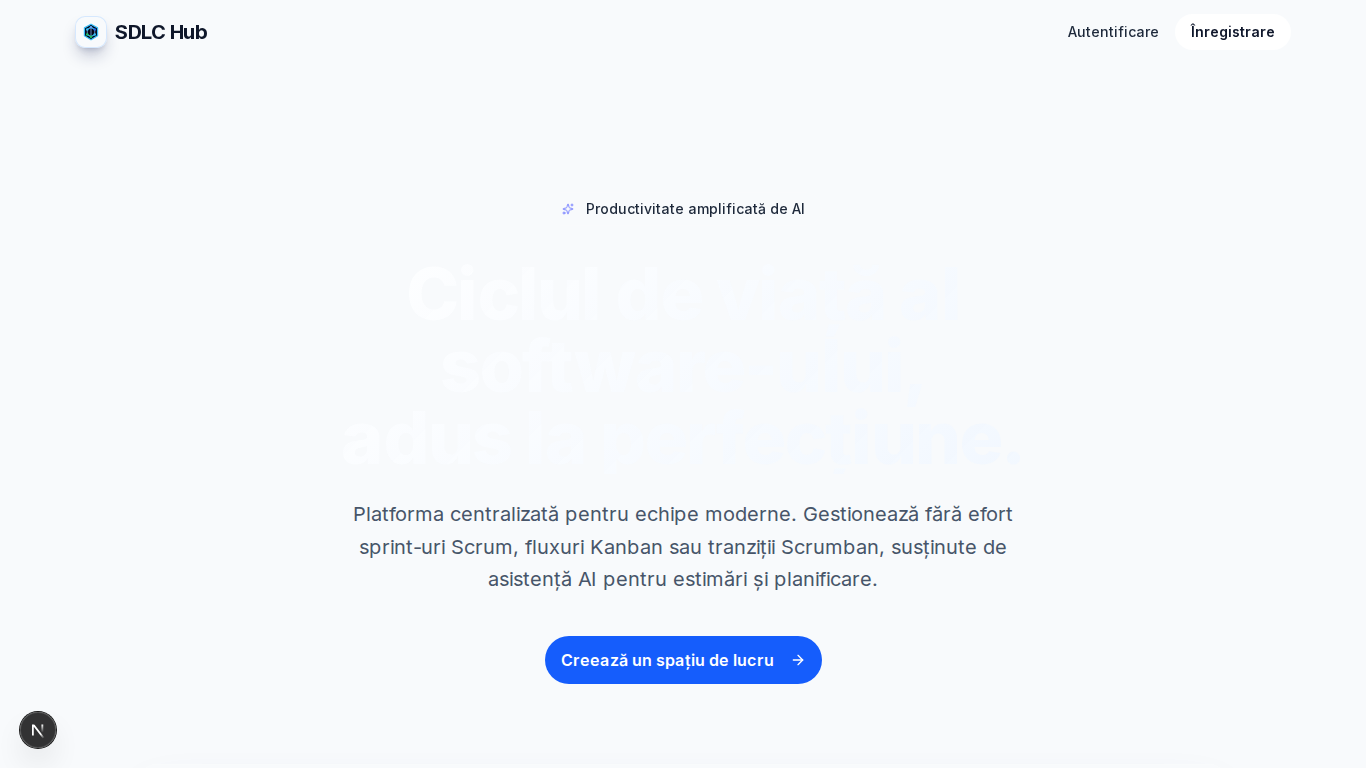
\includegraphics[width=0.9\textwidth]{figures/sdlc-landing.png}
\caption{Landing Page SDLC Hub}
\label{fig:screenshot-landing}
\end{figure}

\begin{figure}[H]
\centering
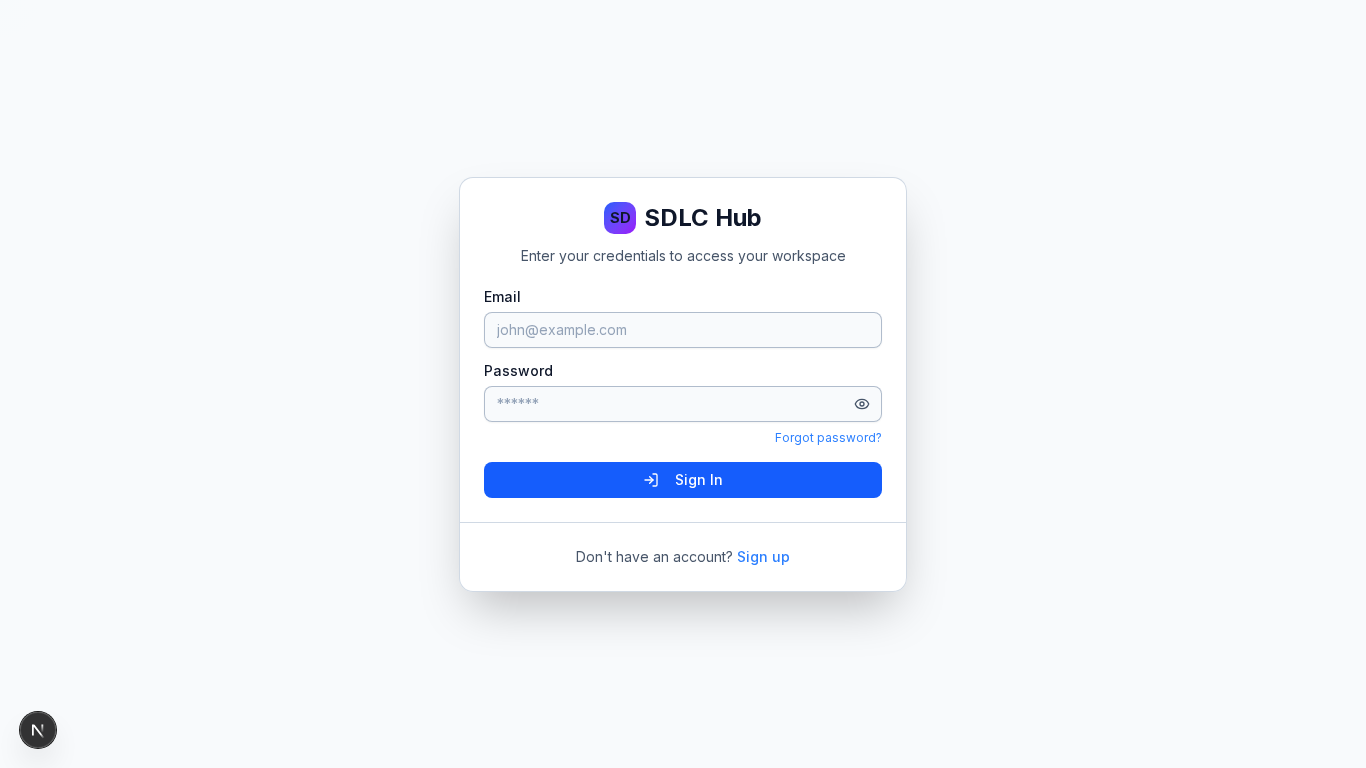
\includegraphics[width=0.9\textwidth]{figures/sdlc-login.png}
\caption{Login Page}
\label{fig:screenshot-login}
\end{figure}

\begin{figure}[H]
\centering
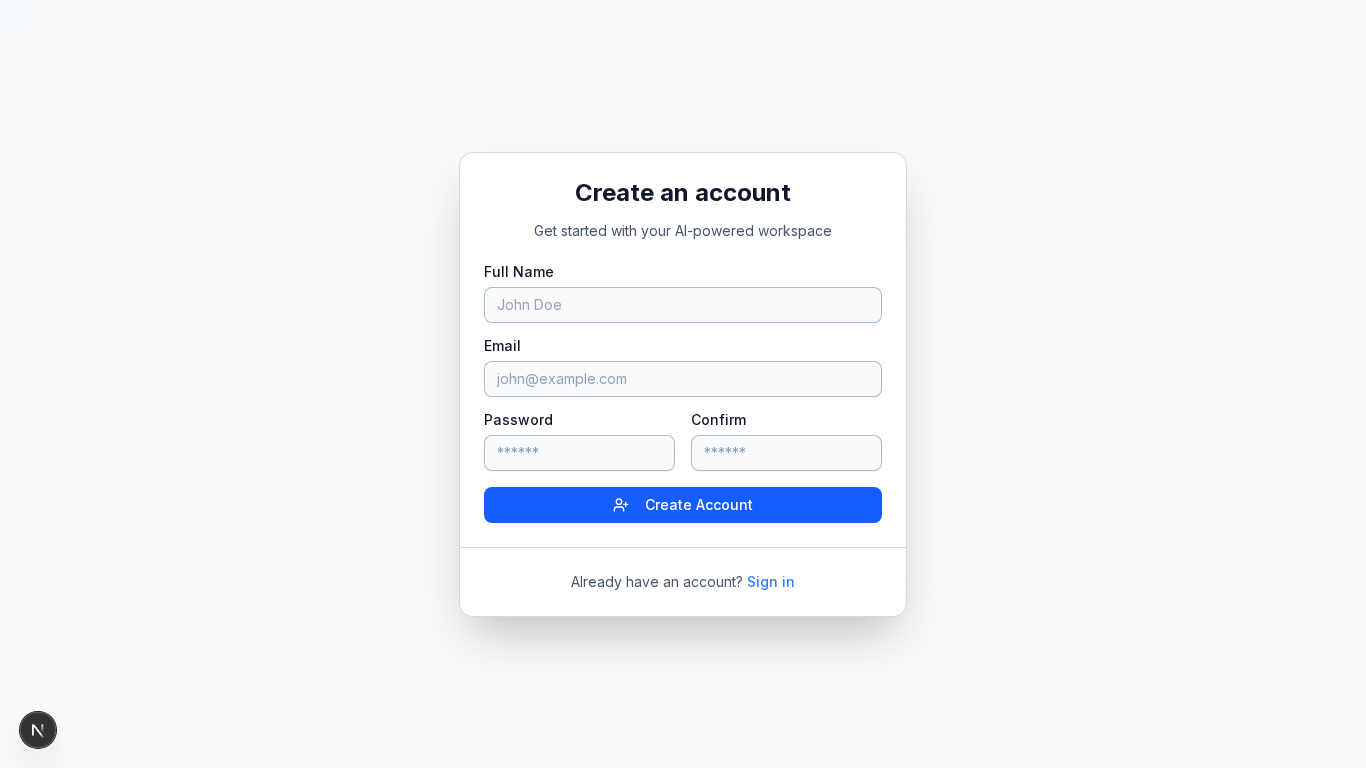
\includegraphics[width=0.9\textwidth]{figures/sdlc-register.png}
\caption{Register Page}
\label{fig:screenshot-register}
\end{figure}

\begin{figure}[H]
\centering
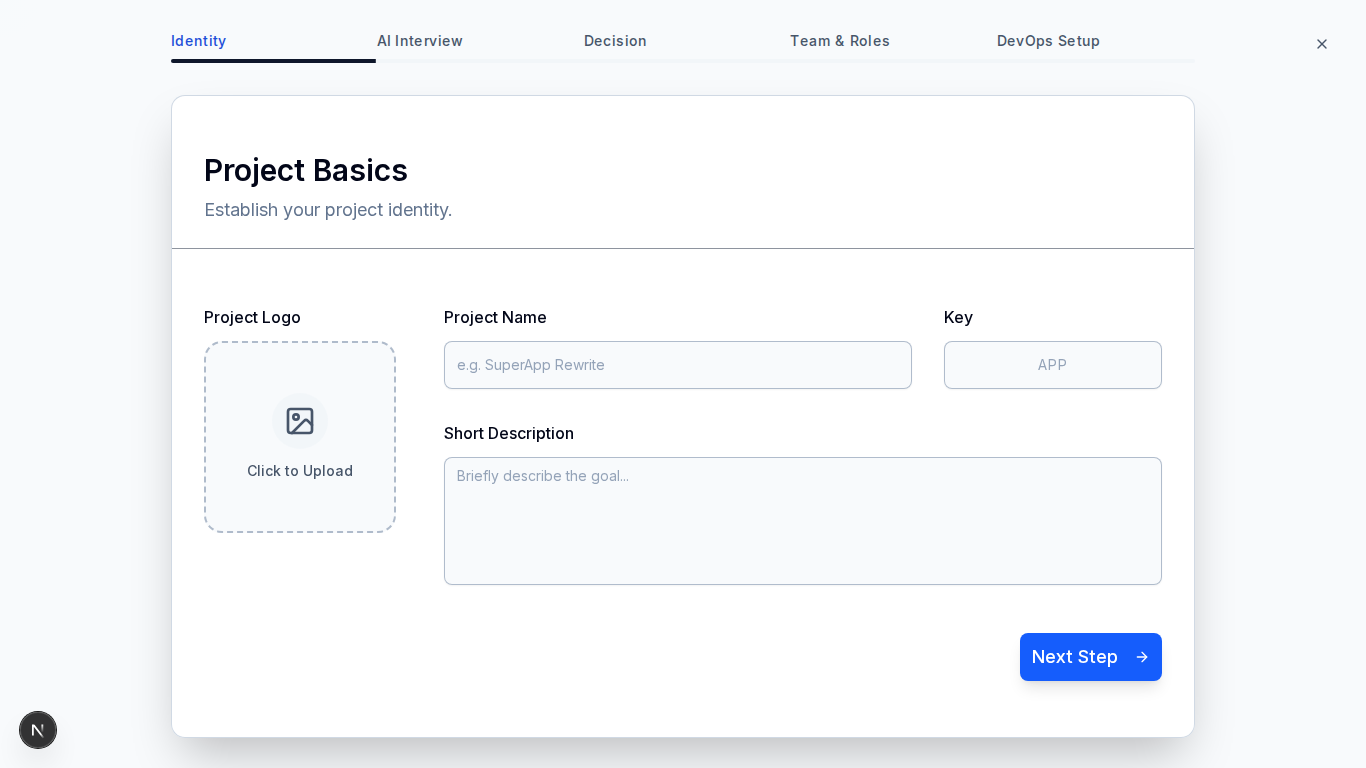
\includegraphics[width=0.9\textwidth]{figures/sdlc-project-wizard.png}
\caption{Project Wizard}
\label{fig:screenshot-project-wizard}
\end{figure}

\begin{figure}[H]
\centering
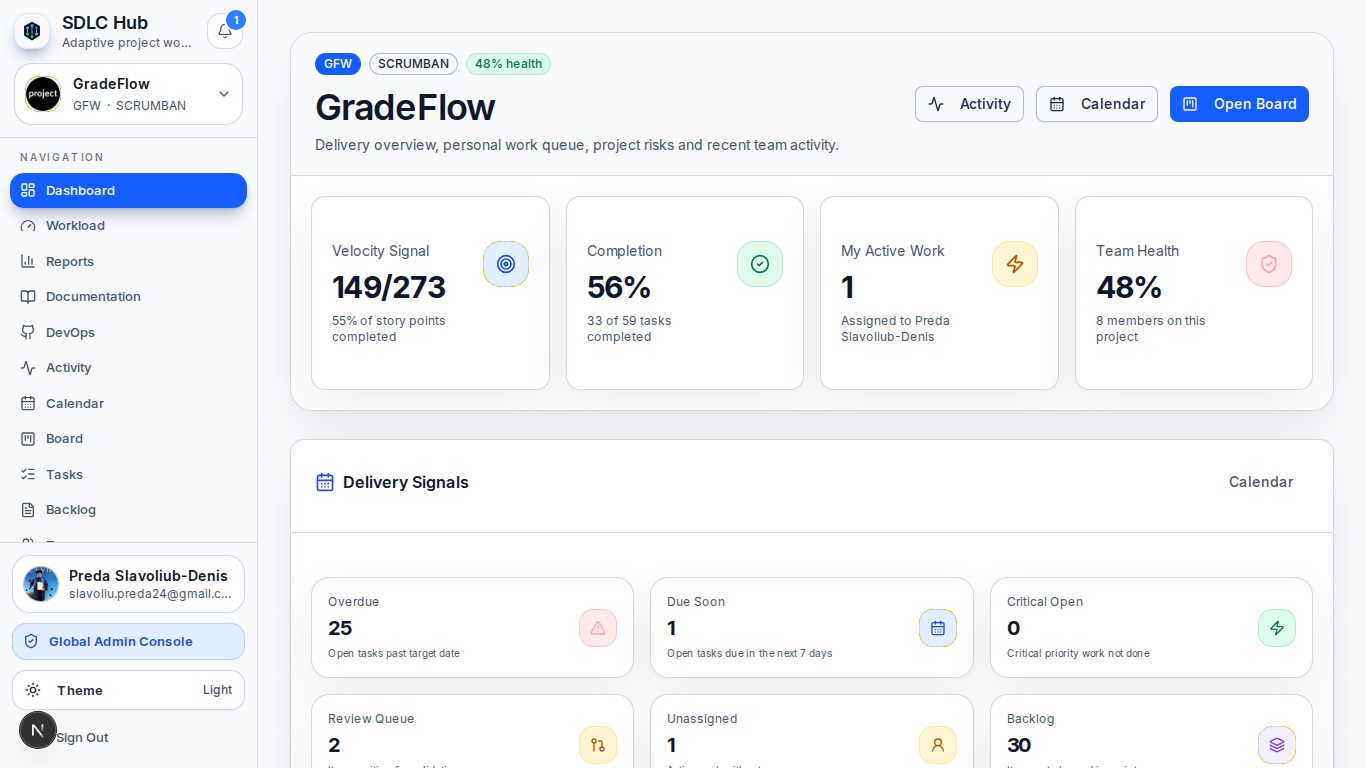
\includegraphics[width=0.9\textwidth]{figures/sdlc-dashboard.png}
\caption{Dashboard Page}
\label{fig:screenshot-dashboard}
\end{figure}

\begin{figure}[H]
\centering
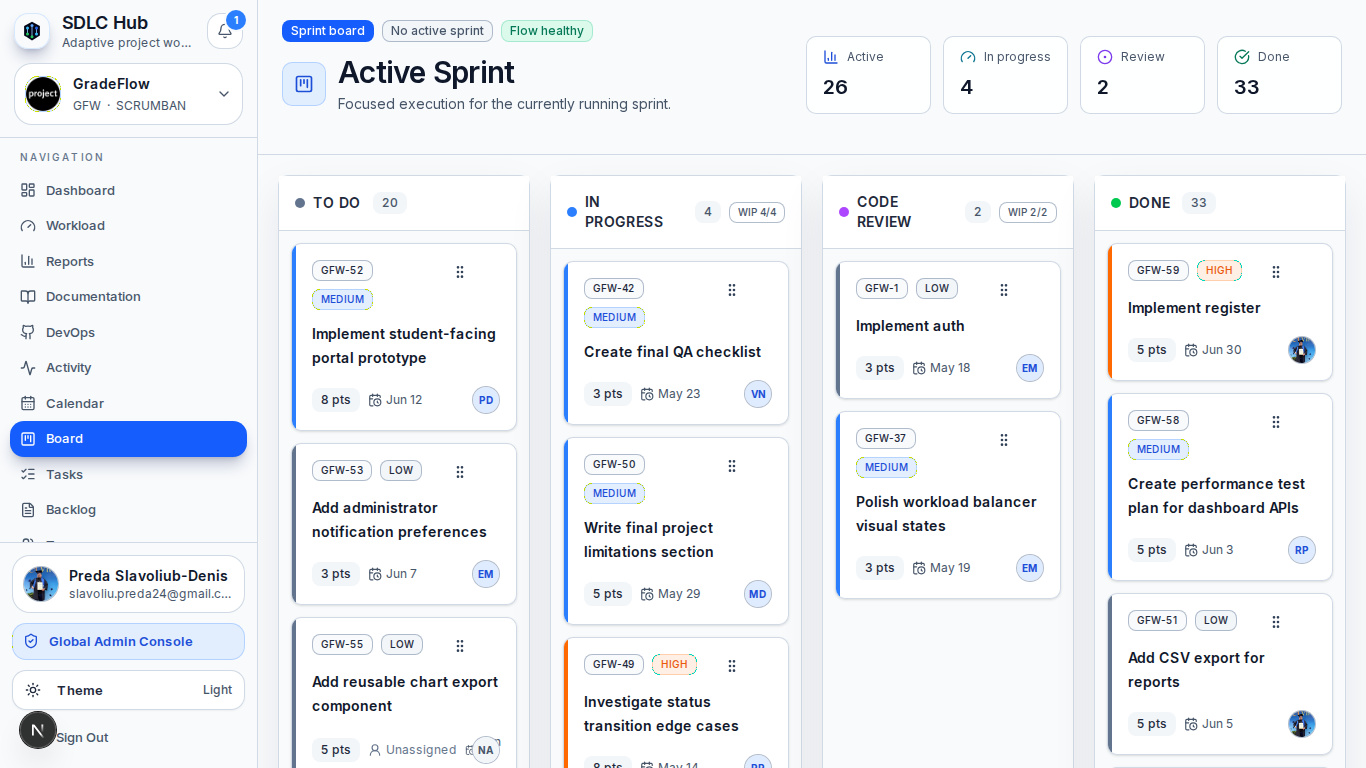
\includegraphics[width=0.9\textwidth]{figures/sdlc-board.png}
\caption{Board Page}
\label{fig:screenshot-board}
\end{figure}

\begin{figure}[H]
\centering
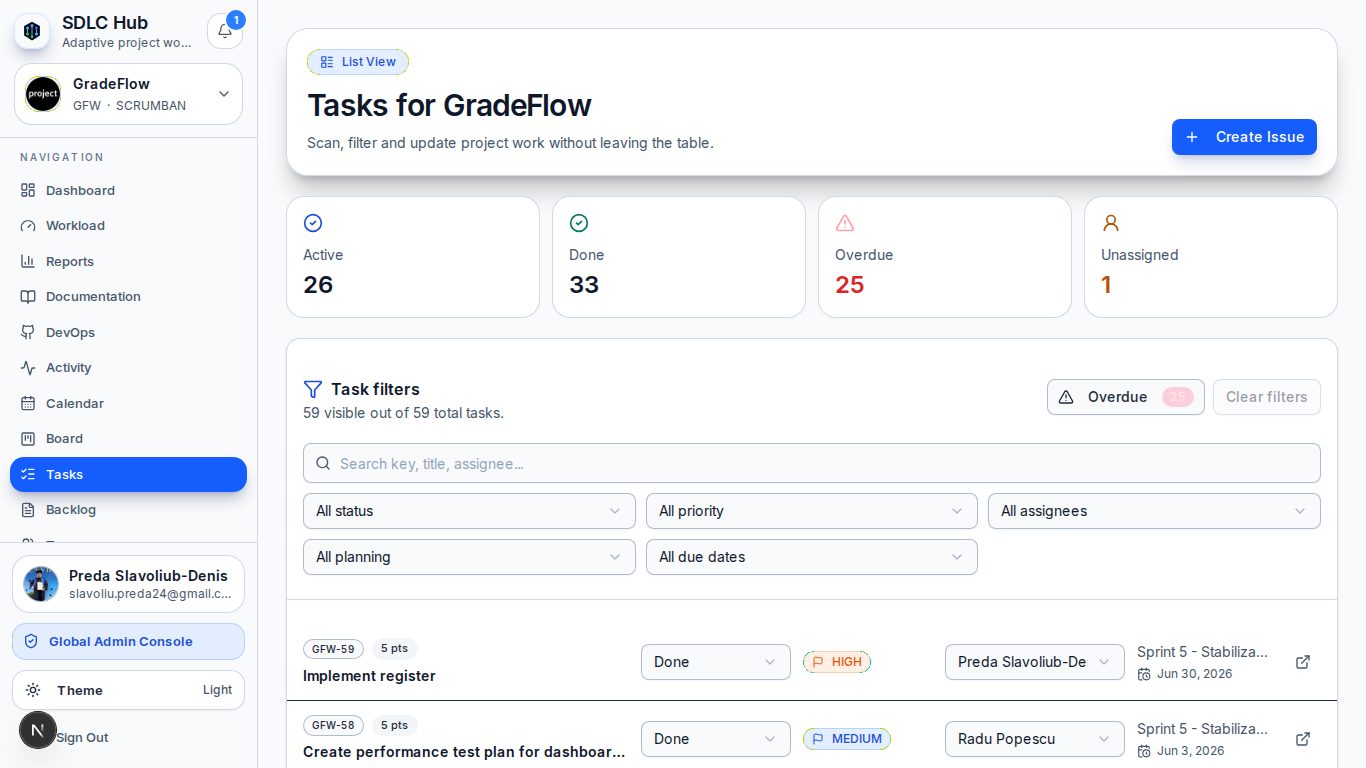
\includegraphics[width=0.9\textwidth]{figures/sdlc-tasks.png}
\caption{Tasks Page}
\label{fig:screenshot-tasks}
\end{figure}

\begin{figure}[H]
\centering
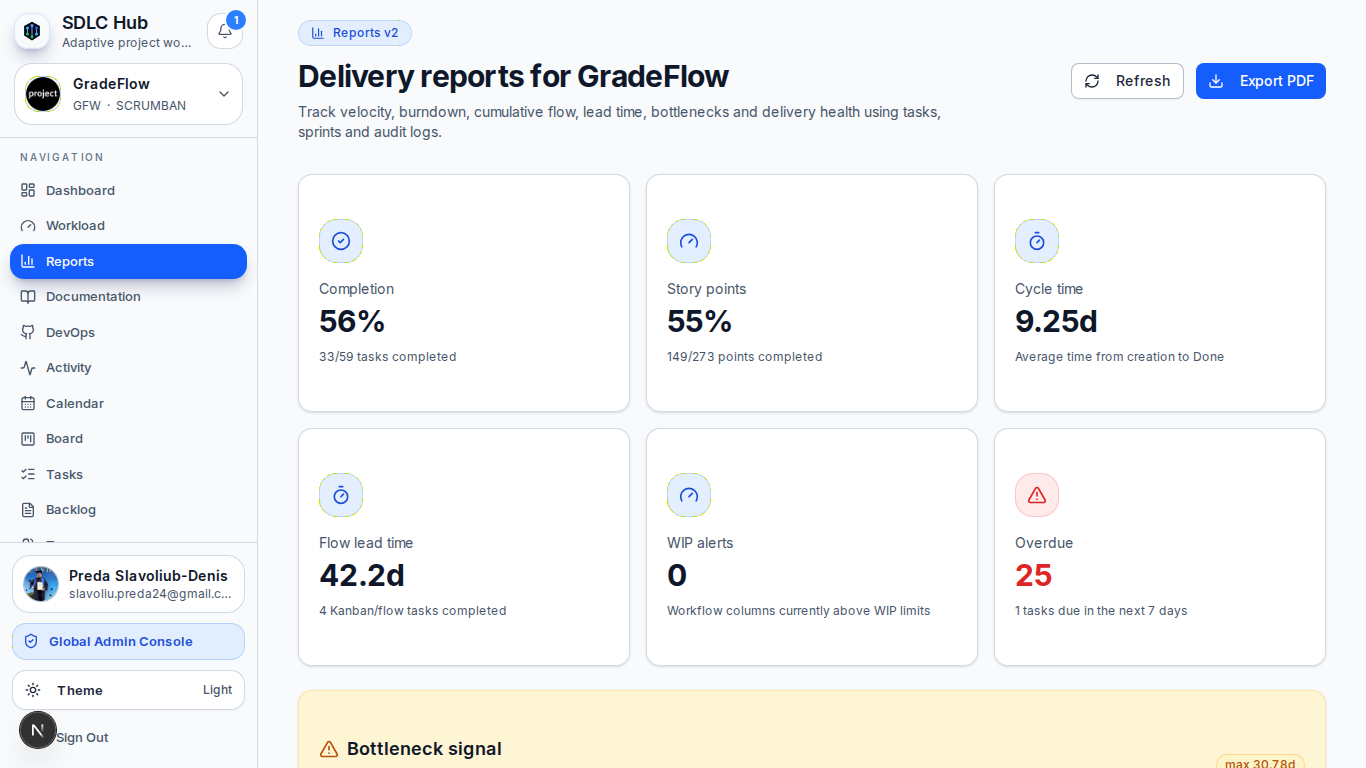
\includegraphics[width=0.9\textwidth]{figures/sdlc-reports.png}
\caption{Reports Page}
\label{fig:screenshot-reports}
\end{figure}

\begin{figure}[H]
\centering
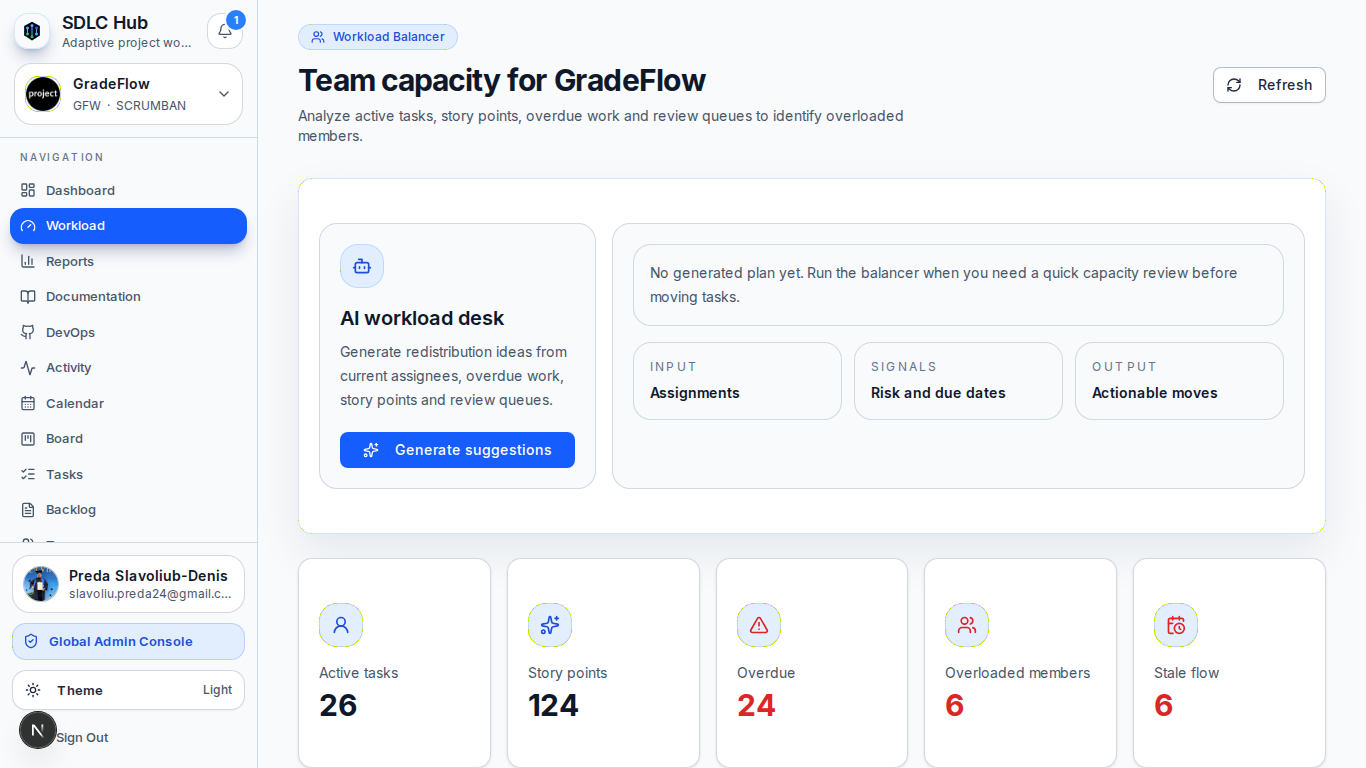
\includegraphics[width=0.9\textwidth]{figures/sdlc-workload.png}
\caption{Workload Page}
\label{fig:screenshot-workload}
\end{figure}

\begin{figure}[H]
\centering
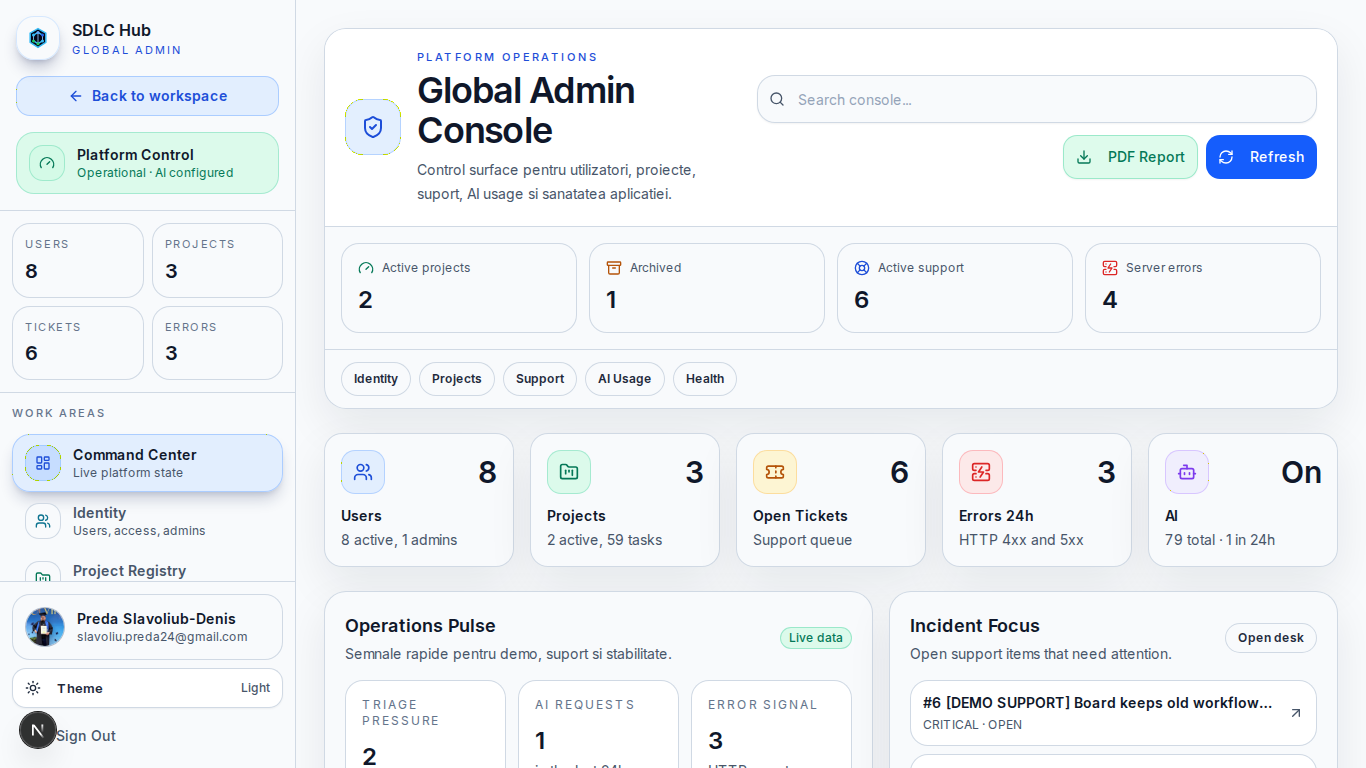
\includegraphics[width=0.9\textwidth]{figures/sdlc-admin.png}
\caption{Admin Console}
\label{fig:screenshot-admin}
\end{figure}

\clearpage
\subsection{Testare}
Pentru a verifica funcționarea aplicației au fost realizate teste manuale și verificări automate headless. Au fost parcurse paginile publice, paginile autentificate, fluxurile de autentificare, proiecte, task-uri, sprinturi, board, rapoarte, workload, calendar, notificări, documentație, integrare GitHub și administrare globală.

Testarea a urmărit atât scenarii pozitive, cât și scenarii negative. La autentificare au fost verificate date corecte și date greșite. La proiecte au fost verificate încărcarea proiectelor, schimbarea metodologiei și blocarea tranziției atunci când există un sprint activ. La task-uri au fost verificate creare, editare, mutare, subtasks, comentarii și audit. Pentru GitHub au fost verificate statusul integrării, evenimentele și lista de pull request-uri. Pentru interfață au fost verificate variante desktop și mobile, light mode și dark mode.

\section{Arhitectura aplicației}
Aplicația folosește o arhitectură pe trei niveluri: frontend, backend și bază de date. Acest model separă interfața utilizatorului, logica de business și persistența datelor, ceea ce ușurează dezvoltarea și testarea sistemului \cite{ibmthreetier}.

\begin{figure}[H]
\centering
\diagramplaceholder{Diagrama arhitecturii sistemului va fi adăugată ulterior.}
\caption{Arhitectura sistemului SDLC Hub}
\label{fig:arhitectura-sistem}
\end{figure}

Frontend-ul comunică cu backend-ul prin API REST, iar backend-ul comunică cu PostgreSQL prin SQLAlchemy. Actualizările live sunt transmise prin WebSocket. Integrarea GitHub se face prin webhook-uri verificate HMAC, iar e-mailurile sunt trimise prin SMTP. Funcțiile AI sunt centralizate într-un serviciu backend care poate folosi un provider extern sau un fallback local.

\subsection{Frontend}
Frontend-ul este construit cu Next.js, React, TypeScript și Tailwind CSS \cite{nextjs,react,tailwindcss}. Structura este organizată pe rute, componente și servicii API. Paginile din \texttt{frontend/app} formează ecranele aplicației, componentele reutilizabile sunt păstrate în \texttt{frontend/components}, iar comunicarea cu backend-ul este centralizată în \texttt{frontend/services}. Pentru interacțiuni vizuale sunt folosite biblioteci precum dnd-kit pentru drag and drop \cite{dndkit}, Recharts pentru grafice \cite{recharts} și Tiptap pentru editorul rich text \cite{tiptap}.

O parte importantă a frontend-ului este adaptarea la contextul proiectului. Componentele nu afișează aceleași acțiuni pentru toate metodologiile. Pagina Backlog este ascunsă pentru Kanban, acțiunile de sprint sunt disponibile doar când metodologia le permite, iar câmpurile de estimare sunt tratate diferit în funcție de modul de lucru. TypeScript ajută la păstrarea contractelor de date între serviciile API și componente.

\subsection{Backend}
Backend-ul este construit cu FastAPI \cite{fastapi}. El expune endpoint-uri REST pentru autentificare, proiecte, task-uri, sprinturi, calendar, notificări, documentație, echipe, rapoarte, GitHub și admin global. SQLAlchemy este folosit pentru accesul la baza de date \cite{sqlalchemy}, iar Alembic gestionează migrațiile \cite{alembic}. Autentificarea folosește JWT \cite{rfc7519jwt}, iar verificarea permisiunilor se face la nivel de endpoint.

Backend-ul este responsabil pentru regulile de business. Dacă frontend-ul trimite o cerere pentru crearea unui sprint într-un proiect Kanban, backend-ul refuză operația. Dacă un utilizator încearcă să mute un task fără permisiune, backend-ul returnează eroare. Dacă un webhook GitHub este primit fără semnătură validă, evenimentul nu este procesat. Astfel, aplicația rămâne sigură chiar dacă interfața este ocolită.

\subsection{Baza de date}
Datele sunt persistate în PostgreSQL \cite{postgresql}. Modelul include utilizatori, proiecte, membri, roluri, echipe, task-uri, subtasks, comentarii, sprinturi, audit log-uri, evenimente calendaristice, disponibilitate, notificări, documentație, integrări GitHub, suport tickets, loguri HTTP și loguri de consum AI. Această structură permite păstrarea separată a datelor operaționale, a istoricului și a integrărilor externe.

\begin{figure}[H]
\centering
\diagramplaceholder{Diagrama modelului conceptual de date va fi adăugată ulterior.}
\caption{Modelul conceptual de date}
\label{fig:model-date}
\end{figure}

Relația dintre \texttt{User}, \texttt{Project} și \texttt{ProjectMember} permite ca același utilizator să participe la mai multe proiecte, cu roluri diferite. Astfel, un utilizator poate fi Project Admin într-un proiect și membru obișnuit în altul. Această flexibilitate este necesară într-o platformă multi-proiect, deoarece drepturile nu aparțin utilizatorului în mod global, ci depind de contextul proiectului.

Entitatea \texttt{Task} este legată de mai multe zone ale sistemului. Ea poate aparține unui sprint, poate avea o echipă de livrare, poate genera audit log, poate fi menționată în documentație și poate primi evenimente GitHub. Această poziție centrală justifică faptul că multe module ale aplicației, precum board, reports, workload, documentation și DevOps, pornesc de la starea task-urilor.

\subsection{Tehnologii folosite}
Pentru backend au fost folosite Python, FastAPI, Uvicorn, SQLAlchemy, Alembic, PostgreSQL, JWT și fpdf2. Pentru frontend au fost folosite Next.js, React, TypeScript, Tailwind CSS, componente shadcn/Radix, TanStack Query \cite{tanstackquery}, dnd-kit, Recharts, Tiptap și Lucide React. Integrarea externă se bazează pe GitHub Webhooks \cite{githubwebhooks}, WebSocket pentru evenimente live \cite{websocketmdn}, SMTP pentru e-mail și ngrok pentru testarea locală a webhook-urilor.

Alegerea acestor tehnologii a urmărit echilibrul dintre productivitate și robustețe. FastAPI permite dezvoltarea rapidă a unui API clar, dar oferă și performanță bună pentru un backend asincron. SQLAlchemy și Alembic oferă control asupra modelului de date și asupra evoluției schemei. PostgreSQL este potrivit pentru relații complexe și pentru integritatea datelor.

Pe frontend, Next.js și React au permis organizarea aplicației pe rute și componente. Tailwind CSS a ajutat la construirea unei interfețe consistente, iar bibliotecile specializate au fost folosite acolo unde era nevoie de comportamente complexe: drag and drop pentru board, grafice pentru rapoarte și editor rich text pentru descrieri și documentație.


\chapter{Concluzii și direcții viitoare}
\label{chap:concluzii}

\section{Concluzii}
Scopul lucrării a fost realizarea unei platforme web de management al proiectelor software, cu suport pentru metodologii diferite și funcționalități asistate de inteligența artificială. Obiectivul a fost atins prin dezvoltarea aplicației SDLC Hub, care oferă fluxuri complete pentru autentificare, proiecte, task-uri, sprinturi, board, roluri, permisiuni, audit, calendar, notificări, documentație, rapoarte, GitHub, realtime și admin global.

Cea mai importantă contribuție este tratarea metodologiei ca parte activă a sistemului. Aplicația nu doar afișează numele metodologiei, ci modifică paginile, regulile, câmpurile și rapoartele în funcție de Scrum, Kanban sau Scrumban. În plus, tranziția între metodologii este făcută controlat, cu preview și audit.

O altă contribuție este integrarea AI în fluxuri practice. AI-ul nu este prezentat ca element decorativ, ci este folosit pentru recomandări, rafinarea cerințelor, estimări, riscuri, workload și release notes. Rezultatele sunt editabile de utilizator, ceea ce păstrează controlul uman asupra deciziilor.

Prin arhitectura aleasă, aplicația separă clar interfața, logica de business și persistența datelor. Această separare a permis integrarea mai multor module fără ca sistemul să devină dependent de o singură pagină sau de un singur flux. Task-urile sunt legate de sprinturi, board, comentarii, audit, documentație și GitHub, iar această legătură oferă trasabilitate pe întregul parcurs al muncii.

Validarea realizată arată că aplicația poate fi folosită pentru scenarii complete de proiect. Au fost testate autentificarea, proiectele, task-urile, sprinturile, schimbarea metodologiei, rolurile, calendarul, notificările, documentația, GitHub, rapoartele și administrarea globală. Rezultatul nu este doar o colecție de ecrane, ci un sistem integrat în care modificările se propagă între module.

Din punct de vedere academic, lucrarea arată cum se poate construi o platformă web care combină concepte de management agile, arhitectură full-stack și funcții asistate de AI. Din punct de vedere practic, SDLC Hub oferă o bază extensibilă pentru echipe care vor să controleze procesul de lucru fără să piardă flexibilitatea metodologică.

\section{Direcții viitoare}
Aplicația poate fi extinsă prin automatizarea mai avansată a testelor end-to-end, astfel încât fluxurile principale să fie verificate constant după fiecare modificare. O altă direcție este integrarea cu calendare externe, precum Google Calendar sau Outlook, pentru ca evenimentele din proiect să poată fi sincronizate cu programul real al membrilor echipei.

Pe partea DevOps, aplicația poate fi extinsă cu integrare GitLab sau Bitbucket, nu doar GitHub. De asemenea, workflow-urile pot deveni mai configurabile, cu reguli mai detaliate pentru tranziții, limite WIP și automatizări. O direcție importantă este și dezvoltarea unor analize mai avansate pentru predictibilitate, risc și capacitate, astfel încât sistemul să poată ajuta echipa nu doar să vadă starea proiectului, ci și să anticipeze problemele înainte ca acestea să afecteze livrarea.

O direcție utilă este dezvoltarea unui sistem de template-uri pentru proiecte. În acest mod, o echipă ar putea porni rapid de la o configurație existentă, cu roluri, workflow-uri, permisiuni și rapoarte predefinite. Template-urile ar reduce timpul de configurare și ar permite reutilizarea unor practici bune între proiecte similare.

Funcțiile AI pot fi extinse printr-un mecanism de feedback. Utilizatorul ar putea marca o recomandare ca utilă sau inutilă, iar sistemul ar putea folosi aceste informații pentru a ajusta prompturile și regulile locale. De asemenea, explicațiile AI ar putea include surse interne din proiect, precum task-uri similare, estimări anterioare sau riscuri întâlnite în sprinturi precedente.

Într-o versiune viitoare, platforma poate include și suport mai avansat pentru organizații. Acesta ar putea adăuga spații de lucru, politici comune, raportare cross-project și management de portofoliu. O astfel de extindere ar păstra principiile aplicației, dar ar permite coordonarea mai multor proiecte în același ecosistem.

\cleardoublepage
\phantomsection
\addcontentsline{toc}{chapter}{Bibliografie}
\bibliographystyle{unsrt}
\bibliography{mybib}

\end{document}
